\documentclass[journal=jpclcd,manuscript=letter]{achemso}
\pdfoutput=1
\usepackage{gensymb}
\usepackage{amsmath}
\usepackage{graphicx}
\usepackage{epsfig}
\usepackage{multirow}
\usepackage{multicol}


% Authors / affiliations
% Authors in alphabetical order except for corresponding author (JJF), need 
% to determine if this is the proper order and if we want to have co-first authors!

\author{Jason Codrington$^{\dagger}$}
\affiliation{Department of Chemistry, William Paterson University, 300 Pompton Road, Wayne, NJ, 07470, USA}
\author{Noor Eldabagh$^{\dagger}$}
\affiliation{Department of Chemistry, William Paterson University, 300 Pompton Road, Wayne, NJ, 07470, USA}
\author{Kimberly Fernando$^{\dagger}$}
\affiliation{Department of Chemistry, William Paterson University, 300 Pompton Road, Wayne, NJ, 07470, USA}
\author{Jonathan J. Foley IV}
\affiliation{Department of Chemistry, William Paterson University, 300 Pompton Road, Wayne, NJ, 07470, USA}
\email{foleyj10@wpunj.edu}

%Title of paper
\title{Unique hot-carrier distributions from scattering-mediated absorption}
% Date
\date{\today}


% Being document
\begin{document}

\begin{tocentry}
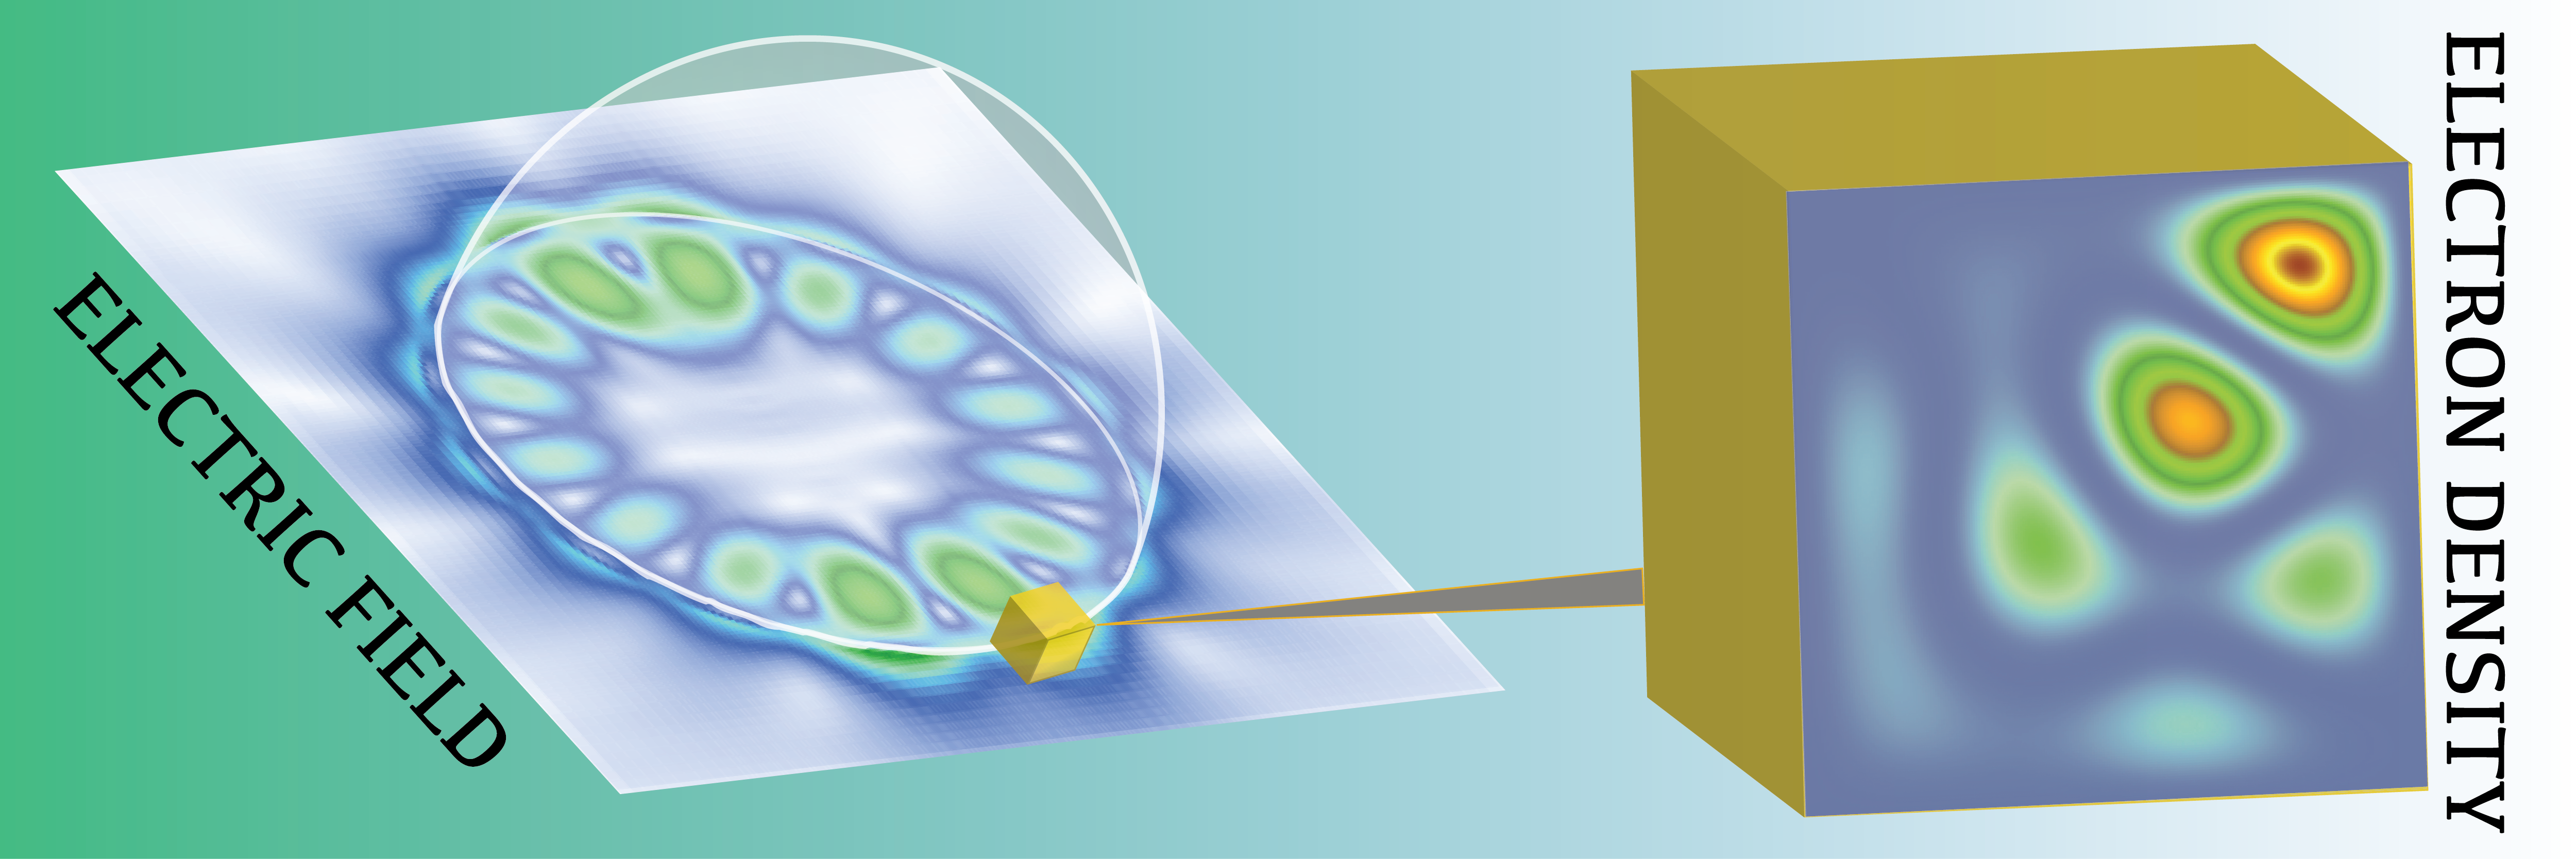
\includegraphics[width=9cm]{figs/nanosphere_WGMv2.png}
\end{tocentry}

\begin{abstract}

Light-initiated generation of energetic carriers has attracted considerable attention as a paradigm for 
photocatalysis and solar energy conversion, and the use of noble metal nanoparticles that support localized surface
plasmon resonances has been widely explored as a medium for realizing this paradigm.  It was recently
shown that composite nanostructures that enable the interplay between dielectric scattering resonances and broad-band
absorption in small metal nanostructures, a phenomenon termed scattering-mediated absorption, can be 
used to mediate energetic carrier transfer and selective photochemistry with 
low-intensity light while completely circumventing plasmon resonance.  In this work, we develop 
a multi-scale modling approach for elucidating the hot-carrier dynamics initiated by scattering mediated
absorption.  Our calculations reveal that unique hot carrier distributions and dynamics arise 
from scattering mediated absorption as compared plasmon excitation, and also suggest that in 
a variety of circumstances, scattering mediated absorption may lead to more
efficienct hot carrier generation than plasmon resonance under the same external illumination
conditions.  These results are an important first step in understanding the phenomena of
scattering mediate hot carrier generation, which has potential for expanding the
pallete of materials that can be utilized for hot-carrier mediated photochemistry,
and for enabling unique pathways for photocatalytic transformations.
\end{abstract}

%%\maketitle

%%\end{document}

\section{Introduction}

Various strategies that exploit the optical properties of metal nanoparticles, namely their ability to support localized surface plasmons resonances (LSPR, which are collective oscillations of their 
conduction electrons driven by visible light), have been explored recently with the aim of using low-intensity light to efficiently drive chemical 
reactions~\cite{LCI_NatureMater_2011,KAC_ACSCatalysis_2013,ZLQ_RSCAdvances_2015,PKL_AccChemRes_2015}.  The interest in this area has 
been motivated partly by the fact that metal nanoparticles (most prominently silver and gold) are exceptionally good absorbers of visible light, 
so they are ideal candidates for harvesting solar photons~\cite{AP_NatMat_2010}.  
Importantly, the resonant properties of plasmonic particles are highly tunable by parameters under synthetic control such as geometry, composition, surface chemistry, and the surrounding 
environment~\cite{SX_Science_2002,BCN_ChemRev_2005,GB_NatPhoton_2010}.  An emerging paradigm that exploits LSPR for photocatalysis is known as Plasmon-mediated Hot-Electron Transfer (PHET),
and a growing number of reports are demonstrating the ability of PHET to catalyze energetically demanding chemical 
reactions~\cite{CXL_NatureChem_2011,MZL_Science_2013,MLL_NanoLett_2013,LFP_AC_2015,ZHX_NatPhoton_2016,ZJM_ACSNano_2016,SZZ_PNAS_2016,SCR_JPCC_2016}.
%There have been several exciting 
%reports that attribute the photocatalysis of energetically demanding reactions to PHET.   This mechanism has been observed to drive the epoxidation of ethylene, a reaction important 
%for the generation of coolants, using silver nanoparticles [18].  Additionally, this mechanism has been observed to lead to the reduction of copper oxide at the surface of 
%copper nanoparticles [19] and reduction of iron oxide at the surface of gold-core iron-shell nanoparticles [20], both of which are important for maintaining the vitality of 
%metal and/or metal oxide catalysts involved in a variety of chemical reactions.   The dissociation of hydrogen adsorbed to gold nanoparticles [21] has also been observed to 
%proceed through PHET, which has implications for using carbon dioxide to create commodity chemicals and chemical fuels.  Importantly, PHET enables many of these reactions 
%under low-light conditions (~1 to 3 suns), which has important implications for using solar energy to drive these reactions.  
In PHET, the collective plasmon excitation decays rapidly (on a ~10 femtosecond timescale) to a non-equilibrium distribution of energetic electron-hole pairs, or a so-called hot-electron 
distribution~\cite{KAC_ACSCatalysis_2013,GZG_JPCC_2013,SNJ_NatComm_2014,WCM_Science_2015,MWW_NatComm_2015, BSN_ACSNano_2016}  
Hot-electrons can deposit energy into reactive degrees of freedom of molecules adsorbed to the nanoparticle surface, thereby initiating chemical transformations.  Despite the considerable progress made in 
demonstrating the potential of the paradigm of PHET, its widespread application faces several challenges. The intrinsic optical properties of noble metals that give rise to the extraordinarily 
large absorption cross sections associated with LSPR are also fundamentally related to the broad energy spectra and short lifetimes associated with LSPR and the subsequent hot-electron 
distributions~\cite{KS_JCP_1983}. 
Furthermore, the timescale of hot-electron relaxation competes 
with transfer to adsorbate states (both occur on 100 fs timescales), which fundamentally limits the efficiency of energy transfer~\cite{WCM_Science_2015}.  Finally, the most promising plasmonic materials typically have poor catalytic activity, and similarly,
good catalytic metals typically are poor light harvesters~\cite{SZZ_PNAS_2016}.

Considering this, an incredible opportunity exists to identify new classes of structures for mediating light-matter interactions and energy transfer events that offer the same advantages as metal nanoparticles, 
namely exceptional light-harvesting potential, while also offering greater selectivity and efficiency in energy transfer, as well as tunable surface chemistry for enhanced catalytic activity.  
Ideally, such structures could be made mostly, if not entirely, from cost-effective materials.  Recent progress towards this aim has been made by designing hybrid 
nanostructures that effectively delegate the light-harvesting and catalytic functions to separate components of the structure.  Recently, Halas and co-workers 
demonstrated an antenna-reactor concept that leverages the near-field enhancement from aluminum plasmons to generate energetic carriers on 
palladium islands and showed the efficacy of this strategy for the photcatalytic transformation of acetylene to ethylene~\cite{SZZ_PNAS_2016}.
Two of the current authors, along with Sun and co-workers, demonstrated a phenomena known as scattering-mediated absorption where dielectric
scattering resonances in SiO$_2$ ionospheres were utilized to induce resonant absorption in non-plasmonic platinum nanoparticles in SiO$_2$/Pt nanohybrids~\cite{ZHX_NatPhoton_2016}.
The scattering-mediated absorption (SMA) phenomena was also observed to induce highly selective photocatalytic oxidation of benzyl alcohol to benzaldehyde~\cite{ZHX_NatPhoton_2016}.
Zhang {\it et al.} independently described a SMA phenomenon in Au-TiO$_2$ nanohybrids that leveraged so-called whispering gallery modes to 
enhance plasmonic and non-plasmonic absorption in gold nanoparticles, and demonstrated these structures efficacy for photocatalytic water splitting~\cite{ZJM_ACSNano_2016}.
Interestingly, hot-carrier transfer was implicated in the photocatalytic mechanisms that resulted from these SMA phenomena~\cite{ZHX_NatPhoton_2016,ZJM_ACSNano_2016}.
The prospect of using SMA in hybrid dielectric/metal nanostructures to initiate hot-carrier generation and transfer is particularly 
compelling as it could completely circumvent plasmon excitation.  Not only does this open up possibilities to utilize a broader palette of materials, it also
presents the possibility of realizing unique photocatalytic pathways owing to differences in the distributions and dynamics of energetic carriers produced by SMA compared
to those produced by plasmon excitation.    

The push to identify novel structures for mediating hot-carrier generation and transfer has been paralleled by 
efforts to develop theoretical methodologies to elucidate these processes.  The underlying electronic
structure has been treated both within free-electron models confined by potential wells~\cite{GZG_JPCC_2013,ZG_JPCC_2014,MLK_ACSNano_2014,KPB_SciRep_2015,SAG_ACSPhotonics_2016} (here called
``particle-in-a-well" (PIW) models), as well as by {\it ab initio} approaches~\cite{SNJ_NatComm_2014,BMN_NatComm_2015,MWW_NatComm_2015,BSN_ACSNano_2016}.
Using PIW models, Govorov and co-workers developed a theory of 
hot-electron generation within the framework of time-dependent perturbation theory that
has elucidated a variety of shape- and size-dependent factors for optimizing 
the hot-carrier generation~\cite{GZG_JPCC_2013,ZG_JPCC_2014}.  A similar approach was also pursued by Kumarasinghe {\it et al.} suggesting
that nanorods are exceptionally good structures for hot-carrier generation~\cite{KPB_SciRep_2015}.  Garc\'ia de Abajo and co-workers recently described a 
quantum master equation approach with an underlying PIW model that elucidated a number of key factors that influence
hot-carrier excitation and decay dynamics~\cite{SAG_ACSPhotonics_2016}.  The utilization of {\it ab initio} approaches by Sundararaman {\it et al} 
has also provided valuable insights into the role that a metals band-structure plays
in determining the efficiency of hot-carrier generation, and particularly in the asymmetry between hot-electron
and hot-hole generation~\cite{SNJ_NatComm_2014}.  Nordlander and co-workers have directly compared free-electron and {\it ab initio} approaches
and found negligible impact on hot-carrier generation and dynamics in Ag nanospheres resulting from electron correlation~\cite{MLK_ACSNano_2014}, 
though Bernardi {\it et al} have demonstrated that many-body effects are important in the hot-carrier dynamics resulting
from surface plasmon polaritons in gold and silver~\cite{BMN_NatComm_2015}.

We develop an novel approach for studying hot-carrier dynamics that may arise from arbitrary electromagnetic
fields, including the unique near-fields that arise from SMA on hybrid dielectric-metal nanoparticles and plasmon resonance
on noble metal nanoparticles.
%In this work, we take a first step towards investigating the unique distributions and dynamics of energetic carriers produced via SMA in 
%dielectric sphere/metal nanoparticle hybrid structures by developing a multi-scale modelling framework
%for simulating the electronic dynamics driven by arbitrary time-domain electromagnetic fields.  We find that the populations
%and dynamics of hot carriers derived from SMA can be tuned through simple
%geometric parameters of the dielectric component of the hybrid structures.   Importantly, we also find that in a variety of circumstances, energetic electron
%generation may be more efficienty by scattering mediated absorption than by plasmon excitation under the same illumination conditions.
We consider the electronic degrees of freedom on the metal nanoparticle subject to the time-dependent Hamiltonian 
\begin{equation}\label{eq:TDHam}
\hat{H}(t) = \hat{H}_{el} - {\bf E}(t) \cdot \hat{\mu}, 
\end{equation}
where the specific form of ${\bf E}(t)$ derives from a rigorous time-domain electrodynamics calculation with a realistic model
of the nanostructures in question and $\hat{H}_{el}$ describes non-interacting electrons confined to metal nanocubes (NCs) an infinite potential well.  
We compute the time-domain field 
using a commercial simulator based on the finite-difference time-domain method~\cite{Lumerical}; more details are given in 
the supplemental information.    

The many-electron wavefunction of the metal nanoparticles is expanded in terms of a configuration-interaction expansion that
includes all singly-excited configurations,
\begin{equation}\label{eq:CIS}
|\Psi_{CIS}\rangle = c_0 |\Phi_0 \rangle + \sum_{i,a} c_i^a |\Phi_i^a\rangle,
\end{equation}
where the configuration $|\Phi_i^a\rangle$ has an electron excited from orbital $i$ to orbital $a$, 
and $c_0$ and $c_i^a$ are complex expansion coefficients.  Unless otherwise specified, indices $i, j$ will indicate
orbitals which are occupied in the ground state reference configuration and indices $a, b$ will indicate orbitals
which are unoccupied in the ground state reference.  

The time-evolution of the wavefunction can be subsumed in the expansion coefficients, which allows the TDSE to be written 
\begin{equation}\label{TDCIS}
i\hbar \frac{ d}{dt} {\bf c}(t) = {\bf H}(t) {\bf c}(t)
\end{equation}
where ${\bf c}(t)$ is the vector of complex expansion coefficients and ${\bf H}(t)$ is the time-dependent Hamiltonian
matrix.  The Hamiltonian matrix is comprised of three unique blocks in the CIS model,  
\begin{equation}
  {\bf H}(t) 
  \mbox{=}
  \begin{pmatrix}
    \langle \Phi_0 | \hat{H}(t) | \Phi_0 \rangle    &     \langle \Phi_0 | \hat{H}(t) | \Phi_i^a \rangle    \\
  \langle \Phi_j^b | \hat{H}(t) | \Phi_0 \rangle    &   \langle \Phi_j^b | \hat{H}(t) | \Phi_i^a \rangle \end{pmatrix}.
\end{equation}
Explicit expressions for Hamiltonian matrix elements are given for both the nanocube and nanosphere models in the supplemental information.
Given the simplicity of the underlying electronic Hamiltonian, the field-free Hamiltonian matrix is diagonal, and only the dipolar
interaction of the nanoparticle with the external field can induce transitions among the electronic configurations, hence the treatment in 
this work neglects excited-state decay contributions from electron-electron scattering.  These contributions will be explored in future work.  Also because of the diagonal nature of field-free Hamiltonian, each configuration $|\Phi_i^a\rangle$ is an eigenfunction
of the field-free Hamiltonian.  This simplifies the interpretation of the electronic structure relative to the CIS 
wavefunction in molecular quantum mechanics where electron repulsion is included in the Hamiltonian
and the excited electronic eigenfunctions are linear combinations of singly-excited configurations. 
The multiplication of the Hamiltonian matrix on the coefficient vector generates the gradient of the coefficient vector in time, and
a variety of algorithms are known that use this information to propagate the wavefunction in time.  Here we use a symplectic integrator
described in Ref.~\citenum{SP_JCP_96}.  Propagation of the CIS wavefunction is referred to as the TDCIS method throughout.

We analyze the hot-carrier distribution and dynamics that results from SMA and plasmon excitation by computing the 
instantaneous populations of orbitals both above and below the Fermi level of the metal nanostructure.   
In our model, the orbitals are energy eigenstates of a 1-electron Hamiltonian and have well-defined kinetic energy,
and the orbital populations are given by the diagonal elements of the 1-electron reduced density matrix,
\begin{equation}
^1D^q_q(t) = \langle \Psi(t) | \hat{a}^{\dagger}_q \hat{a}_q | \Psi(t) \rangle,
\end{equation} 
where the second-quantized operator $\hat{a}_q^{\dagger}$ ($\hat{a}_q$) creates (kills) an electron
in orbital $q$.  The orbital indices can be uniquely mapped to the relevant orbital quantum numbers ($n_x, n_y, n_z$ for
the PIW model for nanocubes) so that the orbital energies can be readily computed. 
%Additionally, each excited state can be mapped to a unique configuration $|\Phi_i^a\rangle 
%Want to emphasize here that the fields themselves are all spatiotemporally distinct.
%Perhaps provide frequency-resolved images here
%Plasmon - short excitation, very broad in energy - provides impulsive kick to the system
%F-P     - moderately short resonance, narrower in energy, provides a more sustained kick to the system
%WGM     - Longer resonance, narrower in energy (many peaks), provides multiple sustained kicks to the system
%        - with repitition times

\begin{figure}
\begin{center}
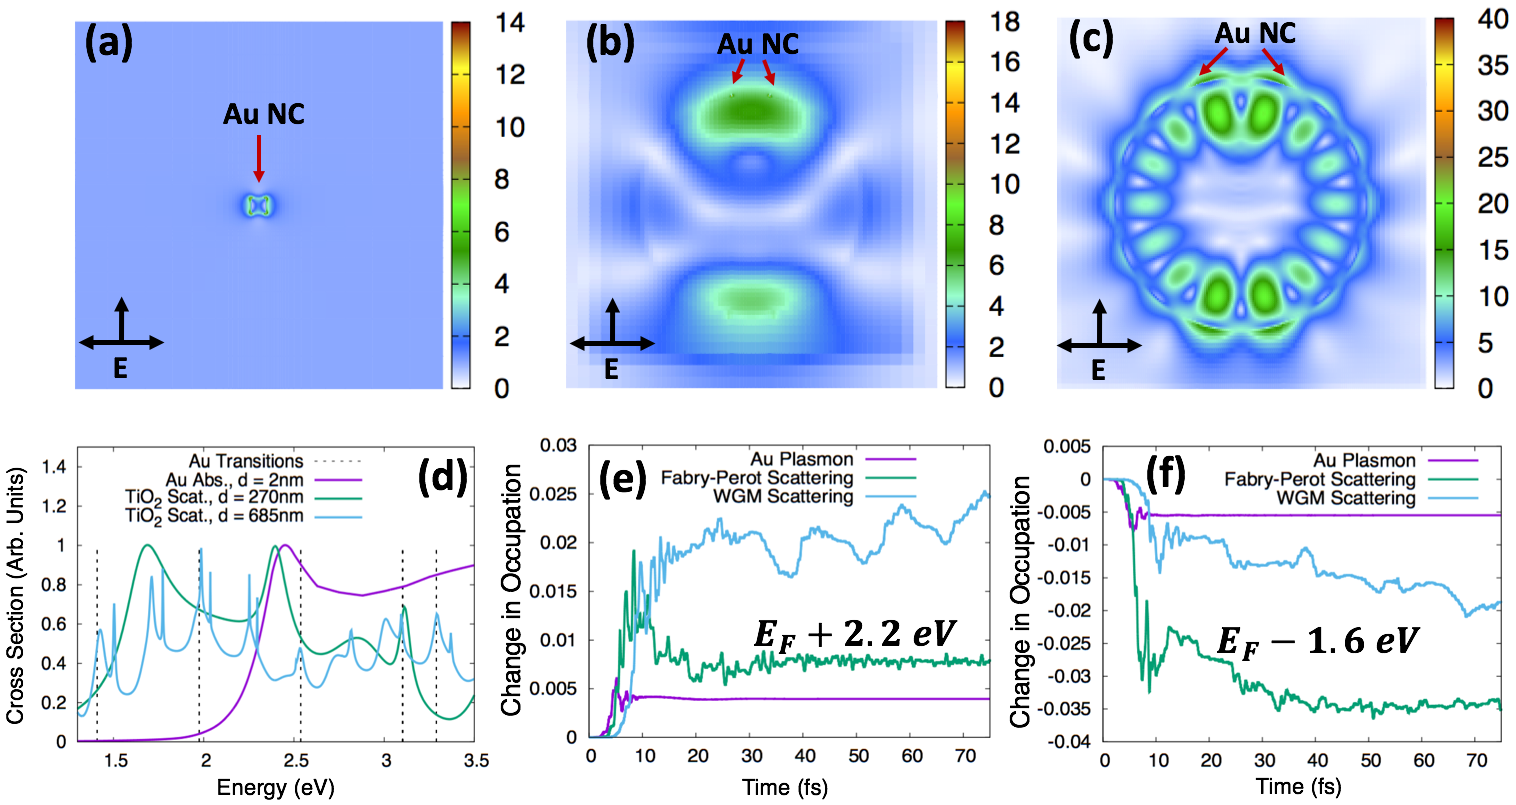
\includegraphics[width=6in]{figs/Au_AllThree_Alternate.png}
\caption{Three regimes for light-matter interactions leading to unique
spatial and temporal shaping of the incident field, and the corresponding
impact on electronic dynamics in a Au nanocube. Plots of the near-field enhancements (${\bf |E|}/{\bf |E_0|}$) are shown of the
Au NC's LSPR ($\lambda=532 nm$, {\bf Panel (a)}), a Fabry-Perot resonance of a d=285nm dielectric NS decorated with Au NCs ($\lambda = 397 nm$, {\bf Panel (b)}),
and a Whispering Gallery Mode resonance of a d=685 nm dielectric NS decorated with Au NCs ($\lambda = 493 nm$, {\bf Panel (c)}).
The extinction spectra of these three structures are shown overlaid with the dipole-allowed transitions in the PIW model of the Au NC, showing particularly
strong overlap between these transitions and the scattering resonances of the d=685 nm dielectric NS ({\bf Panel (d)}).
Both dielectric scattering resonances show more efficient generation of hot-electrons ({\bf Panel (e)}) and hot-holes ({\bf Panel(f)}) compared to LSPR in this case.}
\end{center}
\end{figure}

%% E_f gold is 5.52 eV, Nels = 472
%% E_f Pt   is 9.40 eV, Nels = 1104
Such models of metal (Au and Pt) NCs with $L=2nm$ have a number of dipole-allowed transitions between 1 and 3 eV.
In this work, 4900 singly-excited configurations are included in $|\Psi_{CIS}\rangle$ for both Au and Pt NCs.  The electronic structure
of these model nanocubes is distinguishable by their Fermi energies and the number of electrons: the Au NC model has a Fermi energy 
of 5.52 eV (compared to the bulk value of 5.53 eV) and 472 electrons, the Pt NC model has a Fermi energy of 9.40 eV (compared to the bulk
value of 9.75 eV) and 1104 electrons.  Despite the large number of excited states included in our many-electron wavefunctions, the high 
degeneracy of the underlying dipole-allowed transitions leads to a relatively small number of visible spectroscopic lines for the Au (see Figure 1 (d))
and Pt models (see Figure 2 (d)). 

The spectral flexibility of dielectric scattering
resonances allows tuning to overlap with one or more of these transition energies via the nanosphere size; for example,
a $d=270nm$ dielectric NS has a relatively broad scattering resonance (herein referred to as a Fabry-Perot (FP) resonance) that overlaps 
with an Au transition at 3.1 eV, and
a $d=685nm$ dielectric NS has narrow scattering resonances (whispering gallery modes (WGM)) that overlap with multiple transitions between 1.3 and 3.3 eV.
As proxies of the hot-carrier dynamics in the Au NC, we plot the population dynamics of the highest and lowest energy orbitals in our active space, which lie
2.2 eV above and 1.6 eV below the Fermi energy, respectively (Figure 1 (e) and (f)).  Snapshots of the populations of all active
orbitals in the Au NC model at various times are also provided in the supplemental information (see Figure S1).  
We observe that the LSPR generates a relatively small
population of hot-carriers with field-driven dynamics that evolve on a short (~10 fs) timescale.  FP resonance in this
case lead to significantly more efficient hot-hole generation with field driven dynamics that evolve on a moderate (~50 fs) timescale (Figure 1(f)), while
WGM resonances lead to significantly more efficienty hot-electron generation with field drive dynamics that evolve on a much longer (~200 fs) timescale
(Figure 1(e) and Figure 3(b)).

These differences can be attributed in part to the unique ways in which each resonant interaction simultaneously modulates the incident optical
fields in space and in time. An illustration of spatial confinement associated with each resonance can be see in the 
electric field intensity maps at the resonance frequency for the 
Au LSPR (Figure 1(a)), FP resonance (Figure 1(b)), and WGM resonance (Figure 1(c)); all resonances lead to approximately 1 order of
magnitude nearfield enhancement in the vicinity of the Au NC.  While the spatial 
The larger nearfield enhancement associated with the dielectric scattering resonances
compared to the Au NC LSPR is consisistent with the observation that the dielectric scattering lead to more efficient generation
of hot-carriers. A progression of resonance lifetimes can be inferred from the extinction spectra of the Au LSRP, the FP resonance, and the WGM resonance, with 
the Au LSPR having the broadest extinction peak and the shortest lifetime, and the WGM having the narrowest extinction peaks and longest lifetimes.  These
lifetimes 
Longevity of the evolution of the electric field resulting from dielectric scattering resonances are consistent with 
with longer period of population movement from Fermi level and below to higher unoccupied orbitals when compared with surface plasmon 
resonance of Au.  
%This corresponds to hot-hole generation in lowest orbitals and hot electron generation being potentially more 
%efficient in dielectric scattering structures as opposed to surface plasmon resonance. SPR of 2 nm Au nanoparticle isolated 
%demonstrates population dynamic changes that taper off at 10 fs compared to upwards of 70 fs for 270 nm dielectric-Au composite structure and
%685nm dielectric-Au composite structure. Gold has a Fermi energy of 5.53 eV. Additionally, one can see that there are other orbitals that 
%lie below the Fermi level as well as orbitals that lie above the Fermi level. The Fermi level is the energy of the highest 
%occupied molecular orbital of the ground state configuration. In other words, all the orbitals below the 
%Fermi level and at the Fermi level are doubly occupied to be illuminated. Additionally, all the orbitals above the 
%Fermi level are unoccupied. 
 	
The second figure (Figure 4) depicts the scattering spectra of a succession of differently sized dielectric nanospheres 
and their alignment with the gold dipole-allowed transitions. We observe that the nanosphere with diameter 685nm 
has the best alignment with the gold transitions, and similarly, the 685nm nanosphere is also most efficient 
in generating both hot-electrons and hot-holes. 
\begin{figure}
\begin{center}
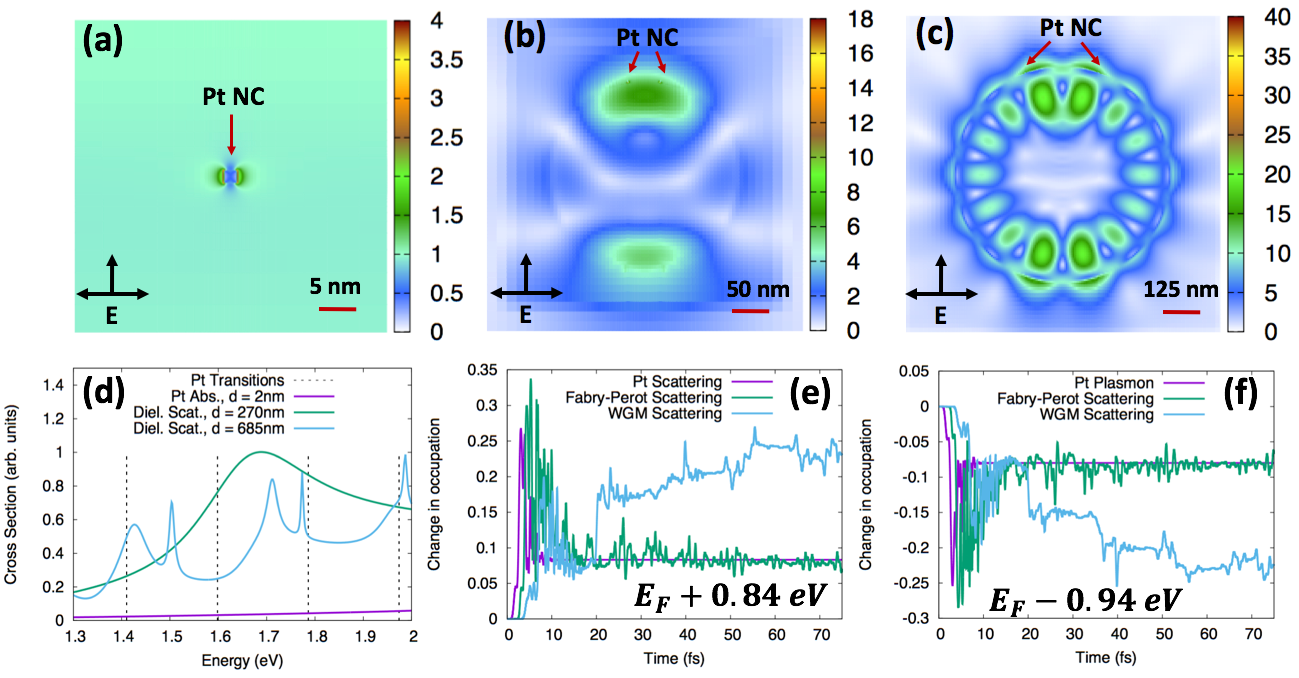
\includegraphics[width=6in]{figs/Pt_AllThree_Alternate.png}
\caption{Three regimes for light-matter interactions leading to unique
spatial and temporal shaping of the incident field, and the corresponding
impact on electronic dynamics in a Pt nanocube. Plots of the near-field enhancements (${\bf |E|}/{\bf |E_0|}$) are shown of the
Pt NC's extinction maximum ($\lambda=200 nm$, {\bf Panel (a)}), a Fabry-Perot resonance of a d=285nm dielectric NS decorated with Pt NCs 
($\lambda = 397 nm$, {\bf Panel (b)}),
and a Whispering Gallery Mode resonance of a d=685 nm dielectric NS decorated with Pt NCs ($\lambda = 493 nm$, {\bf Panel (c)}).
The extinction spectra of these three structures are shown overlaid with the dipole-allowed transitions in the PIW model of the Pt NC, showing particularly
strong overlap between these transitions and the scattering resonances of the d=685 nm dielectric NS ({\bf Panel (d)}).
Both dielectric scattering resonances show more efficient generation of hot-electrons ({\bf Panel (e)}) and hot-holes ({\bf Panel(f)}) compared to LSPR in this case.}
\end{center}
\end{figure}

Figure 5 also represents the scattering spectra of a succession of differently sized dielectric nanospheres and their alignment with 
Pt dipole-allowed transitions. 685nm diameter nanospheres display the most accurate alignment with Pt dipole allowed 
transitions, as was seen in Figure 4 for composite dielectric-Au structures. 

\begin{figure}
\begin{center}
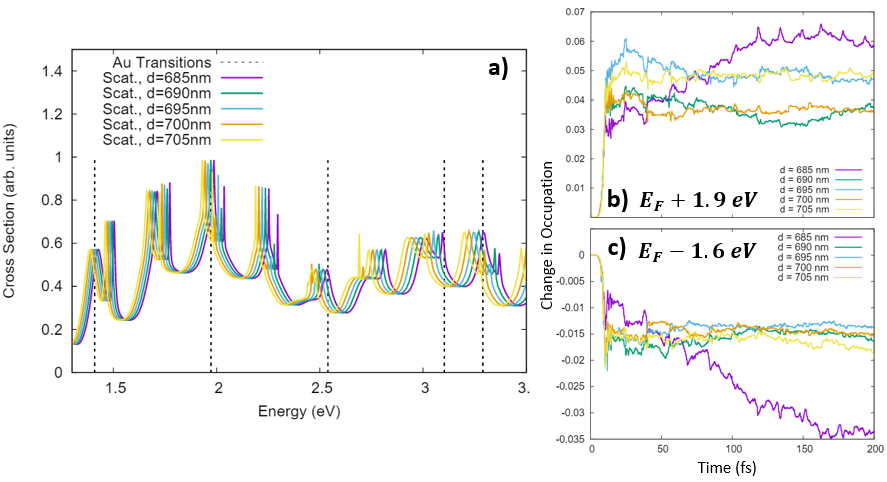
\includegraphics[width=6in]{figs/Au_WGM_Spectrum_and_Trajectories.png}
\caption{Fine-shaping of the spatial and temporal shaping of the incident field
through the geometry of the dielectric nanosphere.  Panel {\bf (a)} shows
the scattering spectra of a size progression of dielectric nanospheres that display
predominately Whispering Gallery Mode visible resonances.  The
685nm nanosphere's scattering spectra has the best overlap with the dipole-allowed
transitions in the Au NC model, and this structure shows most efficient
generation of hot-electrons in the most energetic orbitals included in our
active space (Panel {\bf (b)}), and more efficiently generation of
hot holes in the lowest energy orbitals included in our active space (Panel
{\bf (c)}).   }
\end{center}
\end{figure}
The scattering of the dielectric on the spectra compared with the Platinum transitions has a unique significance when 
compared with the dielectric-Au structure. Although platinum is a non-plasmonic metal in the visible range, it is also 
capable of generating hot-electrons and hot-holes within the visible light range. This demonstrates this method of 
hot electron generation is independent of plasmonic activity and potentially can be expanded to various more abundant and cost efficient metals as opposed to Au. 
The diameter size 685nm is able to excite hot electrons and hot holes on the metal nanocubes on its surface showing its increased 
efficiency over the rest of the sizes. 
Extra figures, to be found in the supplemental information accompanying this paper, show the change in 
occupancy of all the orbitals (with different energies each) in the different structures at various times, 
for the different metals. ( Should we arrange the figures in the supplemental information in groups based 
upon structure, metal {for this paragraph this is how I will arrange them} or time step??) We are able to 
observe in the figures for both metals, that the nano cube structures cease to change their orbital 
occupancy after the 20th timestep. Similarly we find that the Fabry-Perot structures??


\section{Supplementary Information}

\subsection{Plots of Global Hot-Carrier Distributions}

\begin{figure}
\begin{center}
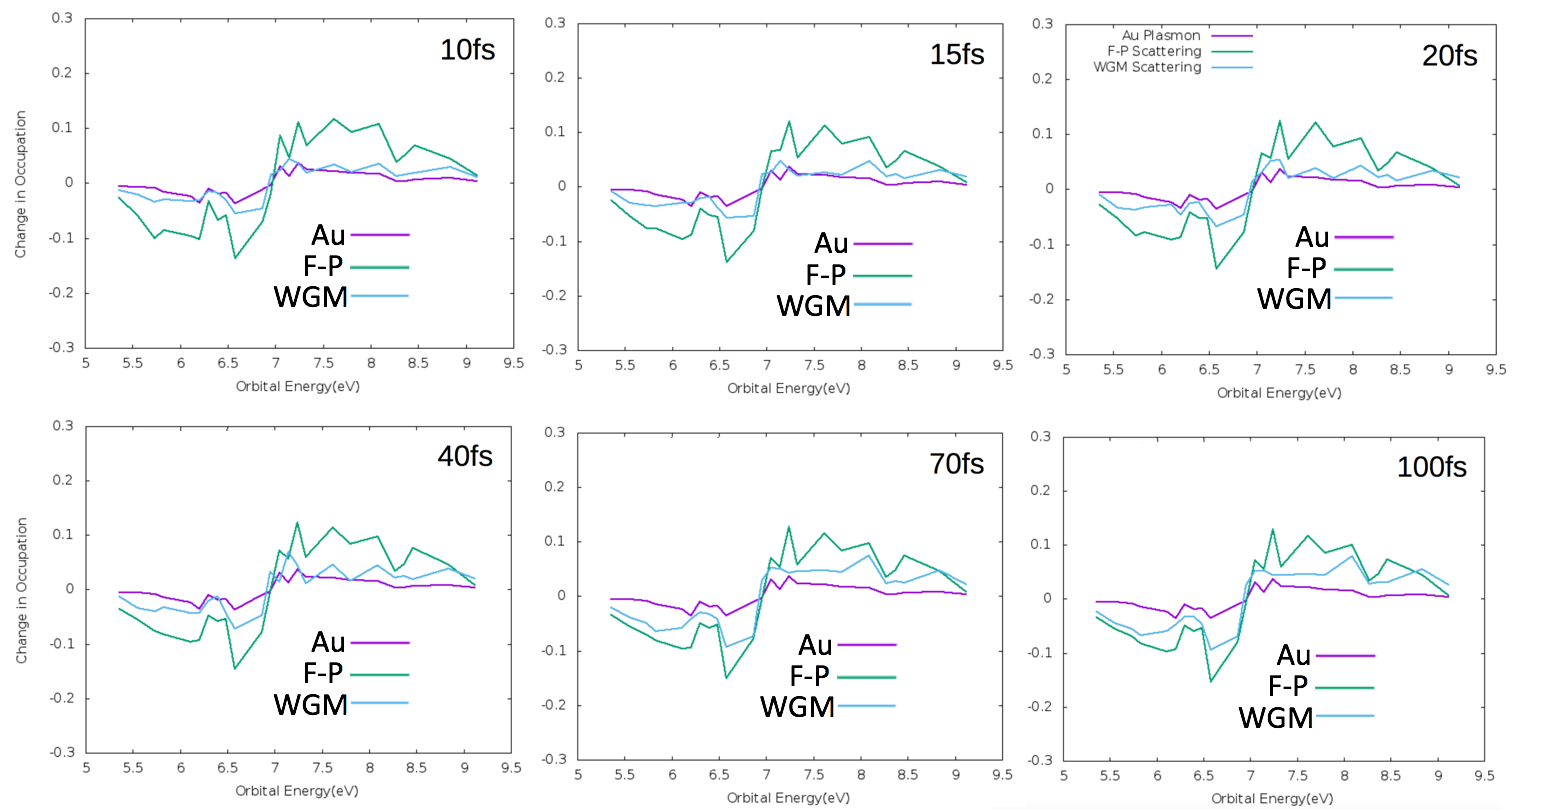
\includegraphics[width=6in]{figs/Au_HotElectronDistribution_Comparison.png}
\caption{Global image of hot-carrier dynamics in Au nanocrystal.}
\end{center}
\end{figure}


\begin{figure}
\begin{center}
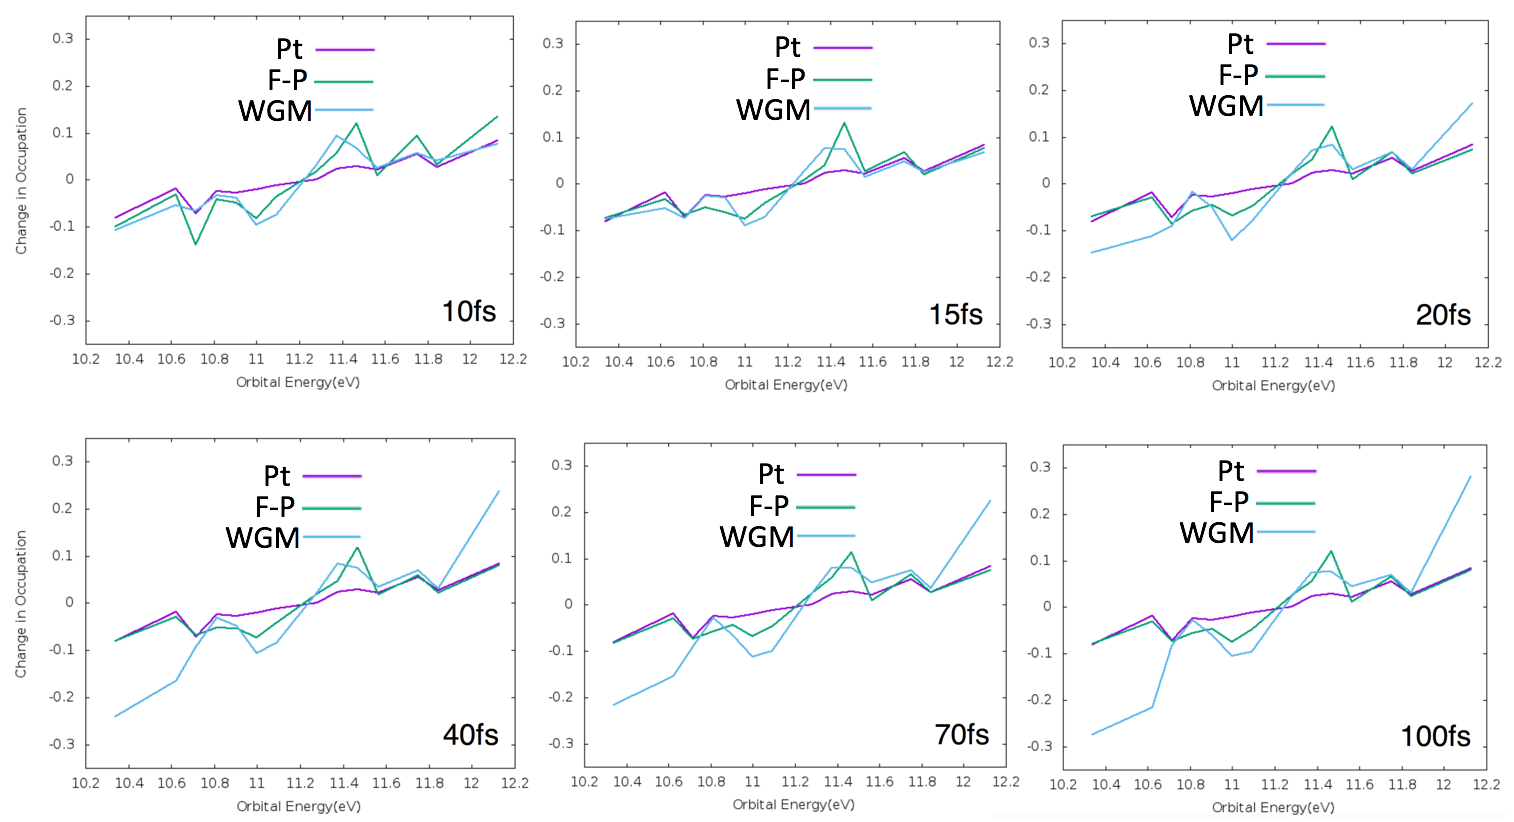
\includegraphics[width=6in]{figs/Pt_HotElectronDistribution_Comparison.png}
\caption{Global image of hot-carrier dynamics in Pt nanocrystal.}
\end{center}
\end{figure}



%\subsection{Time-dependent configuration-interaction singles method}
%We use the time-dependent configuration interaction singles (TD-CIS) method to elucidate the
%electronic dynamics in the metal nanoparticles driven by the electric fields resulting from 
%dielectric scattering resonances, plasmon resonances, or freely propagating light.  
%The TDCIS equations arise directly from the time-dependent Schr\"odinger equation (TDSE) when the wavefunction
%is written as a superposition of a ground state reference configuration, $|\Phi_0\rangle$, and configurations which are singly excited relative
%to $\Phi_0$,  In the CIS model, the wavefunction has the form
%\begin{equation}
%|\Psi_{CIS}\rangle = c_0 |\Phi_0 \rangle + \sum_{i,a} c_i^a |\Phi_i^a\rangle,
%\end{equation}
%where the configuration $|\Phi_i^a\rangle$ has an electron excited from orbital $i$ to orbital $a$, 
%and $c_0$ and $c_i^a$ are complex expansion coeffients.  Unless otherwise specified, indices $i, j$ will indicate
%orbitals which are occupied in the ground state reference configuration and indices $a, b$ will indicate orbitals
%which are unoocupied in the ground state reference.

%Each many-electron configuration is an anti-symmetrized product of one-electron orbitals which are chosen to be energy eigenstates of 
%an appropriate one-electron Hamiltonian, further elaborated in subsequent sections. 
%We neglect electron-electron repulsion in our many-electron Hamiltonian, so the ground state configuration
%can be exactly described by the anti-symmetrized product of the first $N/2$ one-electron orbitals, 
%$|\Phi_0\rangle = |\psi_1 ... \psi_i \psi_j ... \psi_{N/2} \rangle$, where $\psi_q$ denotes the $q^{th}$ one-electron orbital.  

%The time-evolution of the wavefunction can be subsumed in the expansion coefficients, which allows the TDSE to be written 
%\begin{equation}\label{TDCIS}
%i\hbar \frac{ d}{dt} {\bf c}(t) = {\bf H}(t) {\bf c}(t)
%\end{equation}
%where ${\bf c}(t)$ is the vector of complex expansion coefficients and ${\bf H}(t)$ is the time-dependent Hamiltonian
%matrix.  The Hamiltonian matrix is comprised of three unique blocks in the CIS model,  
%\begin{equation}
%  {\bf H}(t) 
%  \mbox{=}
%  \begin{pmatrix}
%    \langle \Phi_0 | \hat{H}(t) | \Phi_0 \rangle    &     \langle \Phi_0 | \hat{H}(t) | \Phi_i^a \rangle    \\
%  \langle \Phi_j^b | \hat{H}(t) | \Phi_0 \rangle    &   \langle \Phi_j^b | \hat{H}(t) | \Phi_i^a \rangle \end{pmatrix}
%\end{equation}
%In our work, the Hamiltonian operator has a component for the electronic energy and a component for a dipolar interaction of the electrons with the electric
%field,
%\begin{equation}
%\hat{H}(t) = \hat{H}_{el} - {\bf E}(t) \cdot \hat{\mu},
%\end{equation}
%and derives time-dependence through the time-dependence of the electromagnetic field that interacts
%with the electrons described by the CIS wavefunction.  Both the electronic and dipolar contributions can be written 
%as sums of one-electron terms %% Probably want to include slater rules... also mention that everything is 1-electron
%The specific forms of the components of the Hamiltonian
%operator are covered in more detail in the following sections. 

%The multiplication of the Hamiltonian matrix on the coefficient vector generates the gradient of the coefficient vector in time, and 
%a variety of algorithms are known that use this information to propagate the wavefunction in time.  Here we use a symplectic integrator
%described in Ref.{\it Sanz-Serna's paper}.



%\subsection{Electronic structure of metal nanospheres}
%For spherical metal nanoparticles, we approximate the one-electron orbitals as energy eigenstates of the particle-in-a-spherical-well. 
%For a particle confined by a spherical well with radius $R$, the potential is 0 when $r<R$ and infinity with $r \geq R$, so that only kinetic energy contributes
%to the energetic.
%The energy eigenstates have the form~\cite{KS_JCP_1983,SKD_Nature_2012} 
%\begin{equation}
%\psi_{n,l,m}(r,\theta,\phi) = j_l(\alpha r) Y_{l,m}(\theta,\phi),
%\end{equation}
%where $j_l(\alpha r)$ are the spherical Bessel functions are 
%$Y_{l,m}(\theta,\phi)$ are the spherical Harmonics.  
%In our numerical implementation, we use the asymptotic approximation of the spherical Bessel functions 
%$j_l(\alpha r) \approx {\rm cos}(\alpha r - \frac{\pi}{2} (l+1))/r$.  To evaluate the spherical harmonics, we use a recursive 
%algorithm described in Ref.~\citenum{Numerical} to evaluate the associated Legendre polynomials.  The energy eigenfunctions
%must vanish at $r=R$, which leads to the following form for the one-electron orbitals:
%\begin{equation}
%\psi_{n,l,m}(r,\theta,\phi)  = 
%\frac{2}{\sqrt{R}} 
%\frac{{\rm cos} \left( \frac{ \pi }{2}(2n + 2 + l)\frac{r}{R} - \frac{\pi}{2}(l+1)\right)}{r} \: Y_{l,m} (\theta,\phi).
%\end{equation}
%The energy eigenvalues have the form 
%\begin{equation}
%E_{n,l} = \frac{\hbar^2 \pi^2}{8 m R^2} \left(2 n + l + 2\right)^2.
%\end{equation}
%From the definition of the spherical polar coordinates, the $x$, $y$, and $z$ components of the transition dipole integrals have the form
%\begin{align}
%\langle \mu_x \rangle =  \int_0^R \int_0^{2\pi} \int_0^{\pi} \psi^*_{n,l,m} \: \hat{\mu}_x \: \psi_{n',l',m'} \:  r^2 \: {\rm sin}\theta \: dr \: d\theta \: d\phi \\
%\langle \mu_y \rangle =  \int_0^R \int_0^{2\pi} \int_0^{\pi} \psi^*_{n,l,m} \: \hat{\mu}_y \: \psi_{n',l',m'} \:  r^2 \: {\rm sin}\theta \: dr \: d\theta \: d\phi \\
%\langle \mu_z \rangle  = \int_0^R \int_0^{2\pi} \int_0^{\pi} \psi^*_{n,l,m} \: \hat{\mu}_z \: \psi_{n',l',m'} \:  r^2 \: {\rm sin}\theta \: dr \: d\theta \: d\phi, 
%\end{align}
%where $\hat{\mu}_x = -e \cdot r \cdot {\rm sin}\theta \: {\rm cos}\phi$, $\hat{\mu}_y = -e \cdot r \cdot {\rm sin}\theta \: {\rm sin}\phi$, 
%$\hat{\mu}_z = -e \cdot r \cdot {\rm cos}\theta$, and $e$ is the charge of the electron.

%In this work, we neglect the $x$ and $y$ components of the field and evaluate $\mu_z$ numerically, where the integral can be
%simplified to
%\begin{equation}
%\langle \mu_z \rangle = \delta_{m,m'} \cdot 2\pi \cdot \int_0^R \int_0^{2\pi} j_{n,l}(\alpha r) \: P_{n,l}({\rm cos} \: \theta) \: \hat{\mu}_z \: j_{n',l'}(\alpha r) \: P_{n',l'}({\rm cos} \: \theta) \: r^2 \: {\rm sin}\theta \: dr \: d\theta,
%\end{equation}
%where $j_{n,l}(\alpha r)$ denotes the asymptotic approximation to the Spherical Bessel Function (written explicitly in Eq. ) and $P_{n,l}({\rm cos} \: \theta)$ denotes
%the associated Legendre polynomial.

\subsection{Electronic structure of metal nanocubes}
For cubic metal nanoparticles, we approximate the one-electron orbitals as energy eigenstates of the particle-in-a-cubic-well.  
For a particle confined by a cubic well with length $L$, the potential is 0 when $x<L, y<L, z<L$ and infinity otherwise.  The energy eigenstates
have the form
\begin{equation}
\psi_{nx,ny,nz} = \left(\frac{2}{L}\right)^{3/2} \: {\rm sin}\left(\frac{n_x \: \pi \: x}{L}\right) {\rm sin}\left(\frac{n_y \: \pi \: y}{L}\right) {\rm sin}\left(\frac{n_z \: \pi \: z}{L}\right).
\end{equation}
The energy eigenvalues have the form
\begin{equation}
E_{nx,ny,nz} = \frac{\hbar^2 \pi^2}{2 \: m \: L^2}\left(n_x^2 + n_y^2 + n_z^2\right).
\end{equation}
The transition dipole integrals can be evaluated analytically,
\begin{align*}
\langle \psi_{nx,ny,nz} |  \hat{\mu}_x | \psi_{nx',ny',nz'} \rangle = e \: \delta_{ny,ny'} \: \delta_{nz,nz'} \:
\frac{L (\pi (n_x - n_x'){\rm sin}(\pi(n_x - n_x'))+{\rm cos}(\pi(n_x-n_x'))-1) }{\pi^2 (n_x - n_x')^2 } \\
-  e \: \delta_{ny,ny'} \: \delta_{nz,nz'} \:
\frac{L (\pi (n_x + n_x'){\rm sin}(\pi(n_x + n_x'))+{\rm cos}(\pi(n_x+n_x'))-1) }{\pi^2 (n_x + n_x')^2 },
\end{align*}
where $\hat{\mu}_x = -e x$.  Analagous expressions can be obtained for expectation values of $\hat{\mu}_y$ and $\hat{\mu}_z$. 

\subsection{Finite-difference time-domain calculations}
A commercial simulator based on the finite-difference time-domain method~\cite{Lumerical} was used to compute the electric field, $E(t)$
1 \AA $\:$  
away from the nanoparticle surface in each of the scenarios considered.  The displacement
was taken along the $z$-axis, corresponding to the polarization direction of incident light since the strongest
near-field enhancement is expected along this direction.  A grid spacking of 1 \AA $\:$  
in $x$, $y$, and $z$ was utilized
in a cubic region extending 1 nm beyond the metal NP surface, and a non-uniform mesh was utilized otherwise with $dx$, $dy$, $dz \leq 20 nm$.
For each composite structure, a nanoparticle was placed at the surface of the dielectric nanosphere at an angle of
20$^{\circ}$ with respect to the propagation axis of the incident light. In all simulations, light propagates
along the $x$ axis and is polarized along the $z$ axis.  The metal nanoparticles are centered at $y=0$.  
A total-field scattered-field source was used to illuminate the structures.  The FDTD simulations were terminated when the 
ratio of the total energy in the simulation volume to the total energy injected by the illumination source falls below
$10^{-6}$.  Because the WGMs are higher quality factor resonances, longer time is typically required for these simulations
as compared to the plasmonic particles alone.  

The resulting time-domain fields were fed into our TDCIS algorithm, allowing us to simulate the electronic dynamics
driven by rigorously-computed nearfields from scattering and plasmon resonances, which show strong spatiotemporal modification relative
to freely propagating light.  The electric field was scaled by a factor $E_0 \approx 614,000,000 \: V/m$ so that the peak power
of the illumination source is $10^{15} \: W/m^2$.  The electric field was sampled at intervals of approximately 2.8 attoseconds for all simulations, which leads
to a time-step that ensures stability of
the wavefunction propagation with the relevant energy scales of our simulations.  Our TDCIS scheme
requires the evaluation of the electric field at intermediate times between these timesteps, and we use a simple update
based on centered-finite differences to approximate the electric fields at these times.  As an example, if the 
electric field is known at times $t_1$, $t_2 = t_1 + dt$, and $t_3 = t_1 + 2\cdot dt$ where $dt = 2.8 \: as$, and knowledge
of the field is required at some time $t_m = t_2 + m\cdot dt$ where $m$ is non-integer, $E(t_m)$ is estimated as follows: 
\begin{equation}
{\bf E}(t_m) =  {\bf E}(t_2) + \frac{{\bf E}(t_3)-{\bf E}(t_1) }{t_3 - t_1 } \cdot m\cdot dt.
\end{equation}

The optical response of Au and Pt in the FDTD simulations utilizes permitivity data from the work of Johnson and Christy~\cite{JC_PRB_1972} and Palik~\cite{Palik}, respectively.  We assume a static dielectric constant of 2.6 for
the dielectric nanospheres in this work, which is comparable to the visible dielectric constant of titanium dioxide. 

\section{Acknowledgment}
This work was performed, in part, utilizing resources at
the Center for Nanoscale Materials, a US Department of Energy, Office of Science, Office of
Basic Energy Sciences User Facility (contract no. DE-AC02-06CH11357).
JJF Acknowledges the College of Science and Health for startup support.
J.C. and N.E. acknowledge the NSF-GS-LSAMP for support.  K.F. acknowledges the WPU CFR for support.
$^{\dagger}$J.C., N.E., and K.F. contributed equally to this work.
\bibliography{SMHET} 

\end{document}
   

